\documentclass[a4paper,12pt]{article} % добавить leqno в [] для нумерации слева
\usepackage[a4paper,top=1.3cm,bottom=2cm,left=1.5cm,right=1.5cm,marginparwidth=0.75cm]{geometry}
%%% Работа с русским языком
\usepackage{cmap}					% поиск в PDF
\usepackage{mathtext} 				% русские буквы в фомулах
\usepackage[T2A]{fontenc}			% кодировка
\usepackage[utf8]{inputenc}			% кодировка исходного текста
\usepackage[english,russian]{babel}	% локализация и переносы

\usepackage{multirow}
\usepackage{graphicx}
\usepackage{mathtools}
\usepackage{wrapfig}
\usepackage{tabularx}
\usepackage{amssymb}
\usepackage{hyperref}
\usepackage[rgb]{xcolor}
\hypersetup{colorlinks=true,urlcolor=blue}
%% Шрифты
\usepackage{euscript}	 % Шрифт Евклид
\usepackage{amsmath}
\usepackage{mathtools}
%%% Заголовок
\author{Lokhmatov Arseniy}
\title{Лабораторная работа по общей физике}

\date{\today}
\begin{document}
\begin{titlepage}
    \newpage
    \begin{center}
    {\large МОСКОВСКИЙ ФИЗИКО-ТЕХНИЧЕСКИЙ ИНСТИТУТ (НАЦИОНАЛЬНЫЙ ИССЛЕДОВАТЕЛЬСКИЙ УНИВЕРСИТЕТ)}
    \vspace{1cm}

    {\largeФизтех-школа аэрокосмических технологий}
    \vspace{6em}
    \end{center}
    
    \vspace{1.2em}

    \begin{center}
    %\textsc{\textbf{}}
    \Large Лабораторная работа №4.3.1 \\
    Излучение дифракционного света
    \linebreak
    \end{center}
    
    \vspace{11em}
    
    \begin{flushright}
                       {\large Работу выполнил\\
                       Лохматов Арсений Игоревич\\
                       Б03-303 }
    \end{flushright}

    \vspace{\fill}

    \begin{center}
        
\includegraphics[width=0.2\linewidth]{dasr.png}
    \end{center}

    \begin{center}
    Долгопрудный, 2025
    \end{center}

    \end{titlepage}

\section{Теоретическая часть}

\paragraph{Цель работы:} исследовать явление дифракции Фринеля и Фраунгофера на одной и двух щелях, изучить дифракции на разрешающую способность оптических инструментов; проверить теоретические соотношения для положения максимумов при дифрауции Френеля и Фраунгофера.

\paragraph{Оборудование:} оптическая скамья, ртутная лампа, светофильтр, щели с регулируемой ши риной, рамка с вертикальной нитью, экран с двойной щелью, микроскоп на поперечных салазках с микрометрическим винтом, зрительная труба.

Схема установки для наблюдения дифракции Френеля представлена на рисунке $\ref{img1}$. Свет от ртутной лампы Л, пропущенной через оранжевый светофильтр Ф со средней длиной волны $\lambda = 578 \text{ нм}$, падает на входную щель $S_1$.
Щель $S_1$ находится в фокусе $\text{коллиматора}$ - собирающей линзы $O_1$. Коллиматор создаёт параллельный пучок монохроматического света, освещающий щель $S_2$, на которой и происходит дифракция. Дифракционная картина рассматривается с помощью микроскопа М, сфокусированного на некоторую плоскость наблюдения П.

\begin{figure}[h]
\begin{center}
    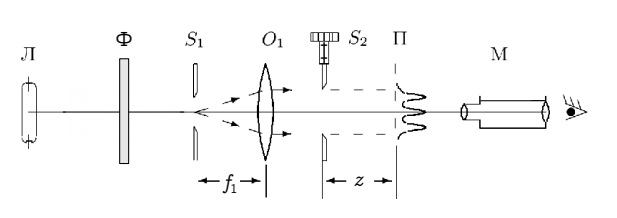
\includegraphics[width=16cm]{установка.png}
\end{center}
    \caption{Схема установки для наблюдения дифракции Френеля}
    \label{img1}
\end{figure}

Распределение интенсивности света в плоскости наблюдения П проще всего рассчитывать с помощью $\text{зон Френеля}$ (для щели их так же называют $\text{зонами Шустера}$). При освещении щели $S_2$ параллельным пучком лучей (плоская волна) зоны Френеля представляют собой полоски, параллельные краям щели (рисунок $\ref{img2}$). 

Результирующая амплитуда в точке наблюдения определяется суперпозицией колебаний от тех зон Френеля, которые не перекрыты створками щели. Границы зон Френеля/Шустера $\xi_m$ определяются соотношением

\[ \xi_m = \pm\sqrt{mz\lambda}, \text{ } m \in \mathbb{N}, \]

где $\xi$ отсчитывается от центра щели, $z$ - расстояние от центра щели до плоскости наблюдения $\text{П}$, а $\lambda$ - длина волны. При ширине щели $b\text{ }(-b/2<\xi<b/2)$ полное число открытых зон для точки наблюдения на оси равно

\[ m=\frac{b^2}{4\lambda z}. \]


По определению, разделение волнового фронта на зоны Френеля производится так, чтобы излучение от соседних зон находилось в $\text{противофазе}$. Иными словами, разность хода (от поверхности фронта до точки наблюдения) между краями соседних зон равна $\lambda/2$. Поэтому, 

\begin{wrapfigure}[16]{l}{0.25\textwidth}
\begin{center}
    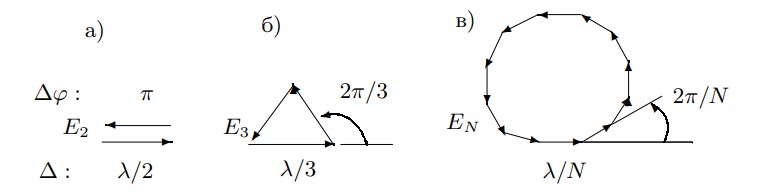
\includegraphics[width=4cm]{image2.png}
\end{center}
    \caption{Зоны Шустерав плоскости щели}
    \label{img2}
\end{wrapfigure}

когда открыто $\text{чётное}$ число зон Френеля, на оси системы наблюдается $\text{минимум}$ дифракционной картины(тёмная полоса). Если число открытых зон $\text{нечётно}$, в центре картины - $\text{максимум}$ (светлая полоса).

Зафиксируем размер щели $b$ и проанализируем, как меняется картина в зависимости от расстояния до плоскости наблюдения $z$. Если чило открытых зон Френеля велико, $m \gg 1 (z\rightarrow0$), мы приходим к пределу геометрической оптики. В нём дифракционная картина отсутствует, а размер изображения щели совпадает с шириной самой щели $b$. Дифракционная картина наблюдается только в узкой полосе вблюзи границ щели (дифракция на краю экрана). При удалении от плоскости геометрического изображения эти две группы полос постепенно расширяются, заполняя всё изображение щелию При $m\sim1$ на щели наблюдается сложная картина из небольшого числа дифракционных полос. При дальнейшем удалении $(m\ll1,\text{ }z\rightarrow\infty)$ дифракционная картина начинается упрощаться и расширяться, переходя в режим $\text{Фраунгофера}$ - затухающие по  интенсивности эквидистантные полосы с характерным угловым размером центральной полосы $\lambda/b$.

Амплитуду света в произвольной точке плоскости наблюдения можно определить графически с помощью векторной диаграммы - $\text{спирали Корню}$.

Распределение амплитуд в режиме дифракции Френеля $(m\sim1)$ довольно сложное. Однако если число открытых зон Френеля больше единицы и близко к целому $(m=2.3...)$, то в картине можно довольно чётко выделить $m-1$ тёмных полос, заполняющих изображение щели. Так можно по виду дифракционной картины оценить число зон Френеля на полуширине щели.

\section{Практическая чать}

\subsection{Дифракция Френеля}

Предлагается исследовать дифракцию Френеля на узкой щели, на краю экрана, на тонкой нити.

\begin{enumerate}
    \item Подготовили приборы к работе:
    \begin{enumerate}
        \item настроили зрительную трубу на бесконечность;
        \item определили нуль микрометрического винта щели $S_2$. Получили $b_0\approx (54.0 \pm 1.0) \text{ мкм}$;
        \item собрали схему согласно рисунку $\ref{img1}$;
        \item проверили, что при небольшом удалении микроскопа от щели на ярком фоне геометрического изображения щели появляются узкие тёмные дифракционные полосы, количество которых уменьшается по мере удаления микроскопа;
        \item Улучшили контрастность картины.
    \end{enumerate}
    \item Добившись наибольшей чёткости и контрастности дифракционной картины, снова нашли резкое изображение щели. Начальное положение микроскопа составляет $l = (68.2\pm0.1)\text{ см}.$.
    \item Постепенно отодвигая микроскоп от щели $S_2$, замеряем по шкале положение микроскопа, при котором на фоне щели видна одна тёмная полоса $(n=1)$. Смещение микроскопа от первоначального положения даёт величину $z$ - расстояние от щели до плоскости наблюдения $(m=n+1)$.
    \item Приближая микроскоп к щели, измеряем зависимость координаты микроскопа $z$ от числа $n$ наблюдаемых минимумов. Результаты измерений представлены в таблице $\ref{tab1}$.

    \begin{table}[h]
        \centering
        \begin{tabular}{|c|c|c|c|c|c|c|}
        \hline
            $n$ & 0 & 5 & 4 & 3 & 2 & 1 \\ \hline
            $m$ & 1 & 6 & 5 & 4 & 3 & 2 \\ \hline
    	$l, \text{ см}$ & 68.2 & 66.9 & 66.6 & 66.3 & 65.5 & 64.5 \\ \hline
    	$z, \text{ см}$ & 0 & 1.3 & 1.6 & 1.9 & 2.7 & 3.7 \\ \hline
        \end{tabular}
    \caption{Результаты измерений}
    \label{tab1}
    \end{table}
    
    \item Измерим ширину $b$ щели $S_2$. Учитывая начальную толщину щели $b_0$, получили $b\approx(402.0\pm1.0)\text{ мкм}.$
    \item Качественные наблюдения:
    \begin{enumerate}
        \item При небольшом удалении микроскопа от щели у её краёв появляются узкие частые полосы. Это $\text{дифракция на краю экрана}$. Возле границы располагалась самая яркая светлая полоса.
        \item для исследования $\text{дифракции Френеля на препятствии}$ мы поставили вместо щели $S_2$ рамку с тонкой вертикальной нитью. Настроили микроскоп на резкое изображение нити. Наблюдаем характерную светлую полосу посередине.
    \end{enumerate}
    \item Обработка результатов:
    \begin{enumerate}
        \item Подобрали координаты так, чтобы зависимость расстояния до щели $z$ от числа открытых зон Френеля $m$ была линейной.Построили график зависимости и с помощью аппроксимации убедились в том, что экспериментальные точки лежат на одной прямой. График представлен на рисунке $\ref{img3}$.
    
    \begin{figure}[h]
    \begin{center}
        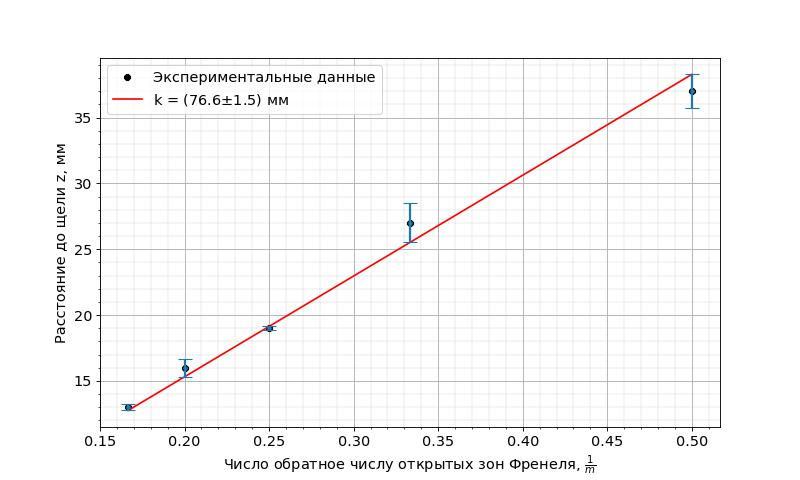
\includegraphics[width=16cm]{image3.jpg}
    \end{center}
        \caption{График зависимости $z\big(\frac{1}{m}\big)$}
        \label{img3}
    \end{figure}

    По наклону прямой определим ширину щели $b$.

    \[ y=z;\text{ }x=\frac{1}{m};\text{ }m=\frac{b^2}{4\lambda z} \Longrightarrow y=\frac{b^2}{4\lambda}x\Longrightarrow k = \frac{b^2}{4\lambda} \Leftrightarrow b = 2\sqrt{k\lambda},\]
    \[\text{ где }\lambda=58\cdot10^{-5}\text{ мм}\text{ - длина волны жёлтого света.} \]
    \[ b=2\sqrt{76.551\cdot58\cdot10^{-5}}=0.420\text{ мм}. \]
    \[ \sigma_{b} = b\sqrt{\Big(\frac{1}{2}\frac{\sigma_{k}}{k}\Big)^2} \Longrightarrow \sigma_{b} = 0.420\cdot\sqrt{\Big(\frac{1}{2}\frac{1.493}{76.552}\Big)^2}=4\cdot10^{-3}\text{ мм}, \text{ }\varepsilon=0.97\%). \]

    \centering\boxed{b=(420\pm4)\text{ мкм}, \text{ }(\varepsilon=0.97\%)}

    \item Сравнили результат с прямым измерением по микрометрическому винту. Отклонение состовляет $\Delta=\frac{420-402}{402}\cdot100\%\approx4\%$.

    \end{enumerate}

\end{enumerate}

\subsection{Дифракция Фраунгофера на щели}

На значительном удалении от щели, когда выполнено условие $m\ll1$ (то есть ширина щели становится значительно меньше ширины первой зоны Френеля $b=\sqrt{\lambda z}$), изображение щели размывается и возникает дифракционная картина, называемая дифракцией Фраунгофера.

Дифракцию Фраунгофера можно наблюдать на той же установке, что и дифракцию Френеля $(\ref{img1})$. Однако при обычных размерах установки дифракцию Фраунгофера возникает только при очень узких щелях. Поскольку работать с тонкими щелями неудобно, для наблюдения дифракции Фраунгофера к схеме добавляется объектив $O_2$ $(\ref{img4})$.

\begin{figure}[h]
\begin{center}
    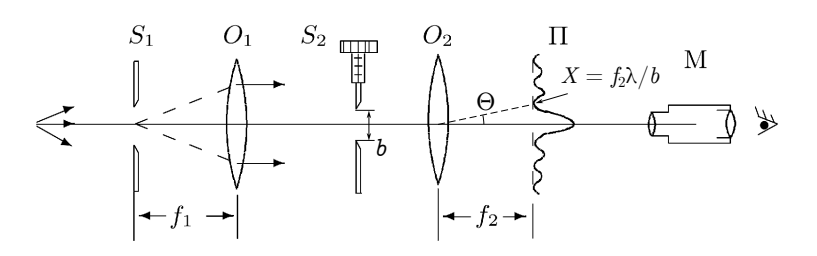
\includegraphics[width=16cm]{image4.png}
\end{center}
\caption{Схема установки для наблюдения дифракции Фраунгофера на щели}
\label{img4}
\end{figure}

Дифракционная картина наблюдается в фокальной плоскости объектива $O_2$. Поскольку объектив не вносит дополнительной разности хода между интерферирующими лучами (\text{таутохронизм} тонкой линзы), в его фольной плоскости наблюдается неискажённая дифракционная картина Фраунгофера, соответствующая бесконечно удалённой плоскости наблюдения.

При дифракции Фраунгофера в центре поля зрения наблюдается дифракционный максимум (светлая полоса). Сбоку от неё наблюдается чередующиеся минимумы и максимумы с довольно быстро затухающей интенсивностью. Направление на минимумы (тёмные полосы) при малых углах $\Theta$ определяется соотношением

\[ \Theta_{n}^{min} = n\frac{\lambda}{b}, \text{ } n=\pm1, \pm2,..., \]

где $b$ - ширина щели. Каждому значению угла $\Theta$ соответствует точка в плоскости объектива с фокусным расстоянием $f_2$, отстоящая от оптической оси на расстоянии

\[ X_{n}=f_2 tg{\Theta_{n}} \approx f_2\Theta_{n}. \]

Измеряя зависимость $X$ от $m$ или расстояние между полосами $\Delta X$, можно определить ширину щели $S_2$.

\begin{enumerate}
    \item Настроили установку:
    \begin{enumerate}
        \item не разбирая схемы из предыдущего управжения, добавили к ней линзу $O_2$ (см. рисунок \ref{img4});
        \item настроили микроскоп на фокальную плоскость $\text{П}$ линзы, закрепили его на скамье;
        \item подобрали ширину щели $S_2$ так, чтобы в поле зрения микроскопа появилась дифракционная картина;
        \item изменили ширину входной щели $S_1$, добившись нвибольшей контрастности картины.
    \end{enumerate}
    \item Провели измерения:
    \begin{enumerate}
        \item С помощью окулярной шкалы микроскопа измерили координаты $x_{m}$ нескольких дифракционных минимумов в обе стороны от центра. Измерения проводили по нижней шкале, цена деления которой составляет $\sigma_{x}=0.04\text{ мм}$. Результаты измерений представлены в таблице $\ref{tab2}$.

    \begin{table}[h]
    \centering
    \begin{tabular}{|c|c|c|c|c|c|c|c|c|c|c|c|c|}
        \hline
            $n$ & -6 & -5 & -4 & -3 & -2 & -1 & 0 & 1 & 2 & 3 & 4 & 5 \\ \hline
            $x_{m}$ & 1.44 & 1.52 & 1.64 & 1.72 & 1.8 & 1.92 & 2.0 & 2.08 & 2.16 & 2.28 & 2.36 & 2.48 \\ \hline
        \end{tabular}
    \caption{Результаты измерений}
    \label{tab2}
    \end{table}

    \item Записали ширину $b$ щели $S_2$ и фокусное расстояние $f_2$ линзы $O_2$. Учитывая ноль микрометрического винта, получили, что $b=(443.5\pm1.0) \text{ мкм}$, $f_2=9\text{ см}$.
    \end{enumerate}
    \item Провели качественные наблюдения. Можно заметить, что:
    \begin{enumerate}
        \item смещение щели $S_2$ в боковом направлениине приводит к сдвигу дифракционной картины. Этот эффект может быть не сильно заметем, если система отцентрирована не точно;
        \item при уменьшении ширины $b$ щели $S_2$ дифракционная картина растягивается.
    \end{enumerate}
    \item Обработали результаты:
    \begin{figure}[h]
        \begin{center}
            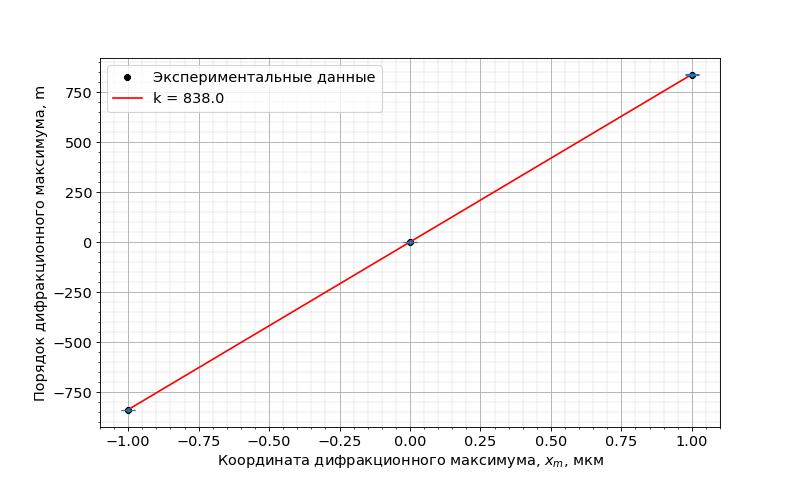
\includegraphics[width=16cm]{image5.jpg}
        \end{center}
            \caption{График зависимости $x_{m}(m)$}
            \label{img5}
        \end{figure}
    \begin{enumerate}
        \item Построили график зависимости положения $x_{m}$ экстремумов дифракционной картины от их номера $m$. Результат представлен на рисунке $\ref{img5}$. Видно, что зависимость может быть аппроксимирована прямой линией.
        \item По наклону прямой определим ширину щели $b$. Оценим погрешность результата.

        \[ y=x_{m{}};\text{ }x=m;\text{ }x_{m}=f_2\frac{\lambda}{b}m \Longrightarrow y=f_2\frac{\lambda}{b}x\Longrightarrow k = f_2\frac{\lambda}{b} \Leftrightarrow b = \frac{f_2\lambda}{k},\]
        \[\text{ где }\lambda=58\cdot10^{-5}\text{ мм}\text{ - длина волны жёлтого света.} \]
    \[ b=\frac{90\cdot58\cdot10^{-5}}{0.093}=0.561\text{ мм}. \]
    \[ \sigma_{b} = b\sqrt{\Big(\frac{1}{2}\frac{\sigma_{k}}{k}\Big)^2} \Longrightarrow \sigma_{b} = 0.561\cdot\sqrt{\Big(\frac{1}{2}\frac{0.001}{0.093}\Big)^2}=3\cdot10^{-3}\text{ мм}, \text{ }(\varepsilon=0.54\%). \]

    \centering\boxed{b=(561\pm3)\text{ мкм}, \text{ }(\varepsilon=0.54\%)}

    \item Сравнили результат с прямым измерением по микрометрическому винту. Отклонение состовляет $\Delta=\frac{561-498}{498}\cdot100\%\approx12\%$.
        
    \end{enumerate}
\end{enumerate}

\subsection{Дифракция Фраунгофера на двух щелях}

Схема для наблюдения дифракции Фраунгофера на двух щелях изображена на рисунке $\ref{img6}$. По сравнению с рисунком $\ref{img4}$ в ней щель $S_2$ заменена на экран $\text{Э}$ с двумя щелями. При этом щель $S_2$ (с микрометрическим винтом) установлена вместо входной щели $S_1$ (для измерения влияния ширины источника на чёткость картины).

Результат дифракции на двух щелях можно представить как $\text{интерференцию}$ дифракционных картин от каждой щели.

\begin{figure}[h]
\begin{center}
    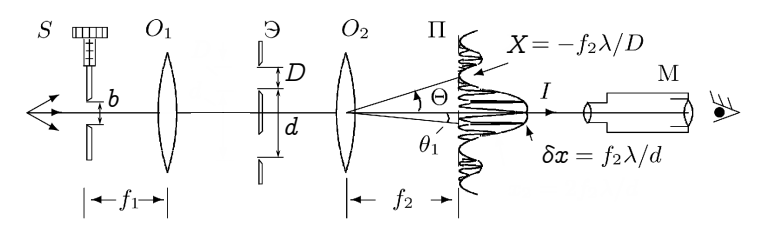
\includegraphics[width=16cm]{image6.png}
\end{center}
\caption{Схема установки для наблюдения дифракции Фраунгофера на двух щелях}
\label{img6}
\end{figure}

Если входная щель достаточно узка, то дифракционная картина в плоскости $\text{П}$ (рисунок $\ref{img6}$) подобна той, что получалась при дифракции на одной щели, однако теперь вся картина испещрена рядом дополнительных узких полос. Наличие этих полос объясняется суперпозицией $(\text{интерференцией})$ световых волн, приходящих в плоскость наблюдения через разные щели экрана $\text{Э}$. В центре главного дифракционного максимума располагается светлая полоса (разность на оси, в силу симметрии, равна нулю). Светлая интерференционная полоса наблюдается также, когда разность хода кратна длине волны.Угловая координата $\Theta_{n}$ интерференционного максимума $n$-ого порядка определяется соотношением

\[ \Theta_{n}d=n\lambda, \text{ }n=\pm1, \pm2,..., \]

где $d$ - расстояние между щелями. Линейное расстояние $\delta x$ между соседними интерференционными полосами в плоскости $\text{П}$ равно

\[ \delta x=f_2\frac{\lambda}{d}. \]

На рисунке $\ref{img6}$ показано распределение интенсивности в фокальной плоскости объектива $O_2$. Штриховой линией изображено распределение интенсивности при дифракции света на одиночной щели. Поскольку полная угловая ширина главного дифракционного максимума (от минимума до минимума) равна $2\lambda/D$, где $D$ - ширина отдельной щели, то на нём укладывается $N=\frac{2d}{D} \text{ тёмных}$ интерференционных полос (в центре картины максимум, поэтому светлых полос - на одну больше).

При дифракции света на двух щелях чёткая система интерференционных полос наблюдается только при достаточно узкой ширине входной щели $S_2$, которую можно рассматривать как протяжённый источник света размером $b$. Для наблюдения интерференции необходимо, чтобы расстояние $d$ между щелями не превышало $\text{радиуса когерентности}$:

\[ d \leq\rho_{\text{ког}} \approx \frac{\lambda}{b}f_1. \]

Таким образом, по рамытию интерференционной картины можно оценить размер источника $b$. Этот метод используется в звёздном интерферометре при изменении угловых размеров звёзд.

\begin{enumerate}
    \item Подготовили установку:
    \begin{enumerate}
        \item Не перемещая линз и микроскопа в установке, убрали входную щель $S_1$ и на её место установили щель с микрометрическим винтом $S_2$. Слегка передвигая щель $S_2$ вдоль скамьи, нашли в микроскопе резкое изображение новой входной щели. Закрепили щель.
        \item Между линзами поставили экран $\text{Э}$ с двойной щелью. В области главного дифракционного максимума появилась система равноотстоящих тёмных и светлых полос (рисунок $\ref{img6}$). Центрировкой системы и подбором ширины входной щели добились наибольшей чёткости дифракционной картины.
    \end{enumerate}
    \item Измерения:
    \begin{enumerate}
        \item Подсчитали число тёмных интерференционных полос в пределах главного (центрального) дифракционного максимума: $N=10$.
        \item Измерили расстояние $\delta x$ между минимумами интерференционной картины: $\delta x=\frac{0.2}{9}=(0.022\pm0.002)\text{ мм}$.
        \item Исследовали влияние размера источника на контрастность интерференционной картины. Для этого, расширяя входную щель $S$, подобрали такую её ширину $b_0=25.5\text{ мкм}$, при которой наступает первое исчезновение интерференционных полос.
        \item При дальнейшем увеличении входной щели картина вновь появляется, но заметно менее контрастна. Соответствующая ширина входной щели равна $b_1=(36.5\pm3)\text{ мкм}$.
        \item Фокусные расстояния линз равны $f_1=12.5\text{ см}$, $f_2=9\text{ см}$.
        \item С помощью микроскопа измерили ширину двойных щелей $D$ и расстояние между ними. Для этого поставили двойную щель непосредственно перед микроскопом:
            \[ D_{11} = 79\cdot0.04=3.16\text{ мм, }D_{12} = 92\cdot0.04=3.68\text{ мм, }\Rightarrow \]
            \[ \Rightarrow D_1=|D_{11}-D_{12}|=(0.52\pm0.02)\text{ мм} -\text{ширина первой щели;} \]
            \[ D_{21} = 155\cdot0.04=6.2\text{ мм, }D_{22} = 162\cdot0.04=6.48\text{ мм, }\Rightarrow\]
            \[\Rightarrow D_2=|D_{21}-D_{22}|=(0.28\pm0.02)\text{ мм} -\text{ширина второй щели.} \]
            \[ d = D_{21}-D_{12}=(2.52\pm0.04)\text{ мм}. \]
    \end{enumerate}
    \item Обработали результаты:
    \begin{enumerate}
        \item По расстоянию $\delta x$ между полосами, рассчитали расстояние между щелями $d$:

        \[ \delta x=f_2\frac{\lambda}{d} \Leftrightarrow d=f_2\frac{\lambda}{\delta x} \Longrightarrow d=90\cdot\frac{58\cdot10^{-5}}{0.022}=(2.37\pm0.21)\text{ мм}. \]

        Полученное значение совпадает по порядку с измеренным. Отклонение составляет $\Delta = \frac{2.52-2.37}{2.52}\cdot100\%\approx6\%.$
        \item Сравнили наблюдаемое число полос в главном максимуме с теоретическим:

        \[ N^{theor}_1 = \frac{2d}{D_1} = \Bigg[\frac{2\cdot2.37}{0.52}\Bigg] = 9,\text{ } N^{theor}_2 = \frac{2d}{D_2} = \Bigg[\frac{2\cdot2.37}{0.28}\Bigg] = 16. \]

        Измеренное число наблюдаемых полос в главном максимуме лежит в диапазоне полученных значений для каждой щели в отдельности. Более точно мы не можем сравнить, так как на это влияет юстировка системы, то есть какая щель даёт больший вклад.

        \item Сравнили измеренную ширину $b_0$ входной щели $S$ с теоретическим расчётом:

        \[ d \leq\rho_{\text{ког}} \approx \frac{\lambda}{b_0}f_1 \Longleftrightarrow 2.52\leq\frac{28\cdot10^{-5}}{25.5\cdot10^{-3}}\cdot125=2.84 - \text{верно!} \]

        \item Рассчитаем ширину $b_1$, при котором изображение должно опять появиться. Для этого рассмотрим предельный случай:

        \[ d =\frac{\lambda}{b_1}f_1 \Longleftrightarrow b_1=\frac{\lambda}{d}f_1 \Longrightarrow b_1=\frac{58\cdot10^{-5}}{2.52}\cdot125=28.8\cdot10^{-3}\text{ мм.} \]

        Полученное значение совпадает по порядку величины с измеренным.
        
    \end{enumerate}
\end{enumerate}

\section{Подведение итогов и выводы}

В данной лабораторной работе мы исследовали явление дифракции Фринеля и Фраунгофера на одной и двух щелях, проверили теоретические соотношения для положения максимумов при дифрауции Френеля и Фраунгофера.

В ходе работы мы научились юстировать сложные оптические системы, работать с линзами и дифракционными щелями, фильтром света.

Исследовали зависимость расстояния до щели $z$ от числа открытых зон Френеля $m$ (рисунок \ref{img3}), с помощью графика определили размер щели $b$; исследовали зависимость положения экстремумов $x_m$ от их номера $m$ (рисунок \ref{img5}), с помощью графика определили размер щели $b$.

Полученные значения совпадают по порядку величины с теоретическими, и во всяком случае не противоречат здравому смыслу. Отклонения могут быть связаны с неточной юстировкой системы.



\end{document}
